\section{Tuning}

Your guitar needs to be in tune. This means that each string has a certain pitch. Even though this is already implied, it is important to note that the relative pitch different per string is important as well.

In \ref{fig:guitar_string_names} you see the names (letters) from the thinnest (\textit{e}) to the thickest (\textit{E}) string.

\begin{figure}[h]
    \centering
    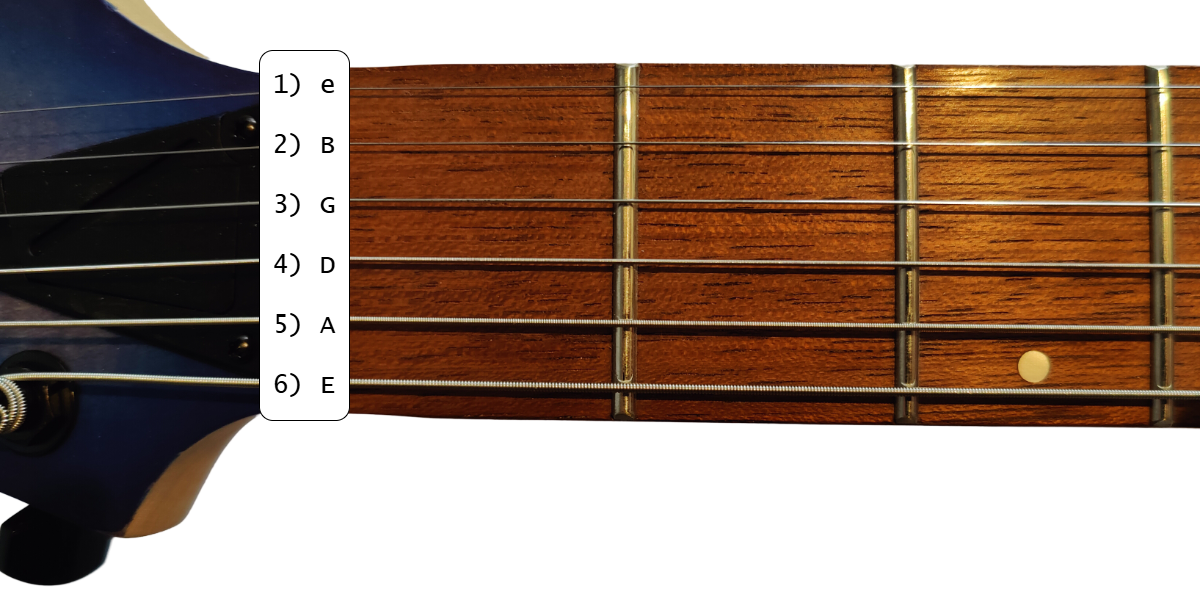
\includegraphics[width=0.5\textwidth]{../Images/guitar-neck-string-names.png}
    \caption{Names of the guitar strings}
    \label{fig:guitar_string_names}
\end{figure}

A mnemonic is (from low/thick to high/thin):

 \begin{minipage}{0.25\textwidth}
    \vspace{3mm}
    \begin{itemize}
        \setlength\itemsep{0em}
        \item[6)] \textbf{E} ddie
        \item[5)] \textbf{A} te
        \item[4)] \textbf{D} ynamite
        \item[3)] \textbf{G} ood
        \item[2)] \textbf{B} ye
        \item[1)] \textbf{e} eddie 
    \end{itemize}
    \vspace{3mm}
\end{minipage}
\hfill
\begin{minipage}{0.7\textwidth}
    \infobox{Note that things is the standard tuning. Sometimes the guitar will be tuned differently. But that will then be explicitly mentioned}
\end{minipage}

\begin{minipage}{0.5\textwidth}
You use a tuner to tune (see \ref{fig:tuning}). The tuner either gives a note value, and then you have to tune up or down to get the correct note on the screen. Or it shows a string number and you have to get the 'pointer' in the middle.

Be careful with tuning the string up (to a higher pitch). Especially the thinner strings can break if they are too right.
\end{minipage}
\hfill
\begin{minipage}{0.34\textwidth}
    \centering
    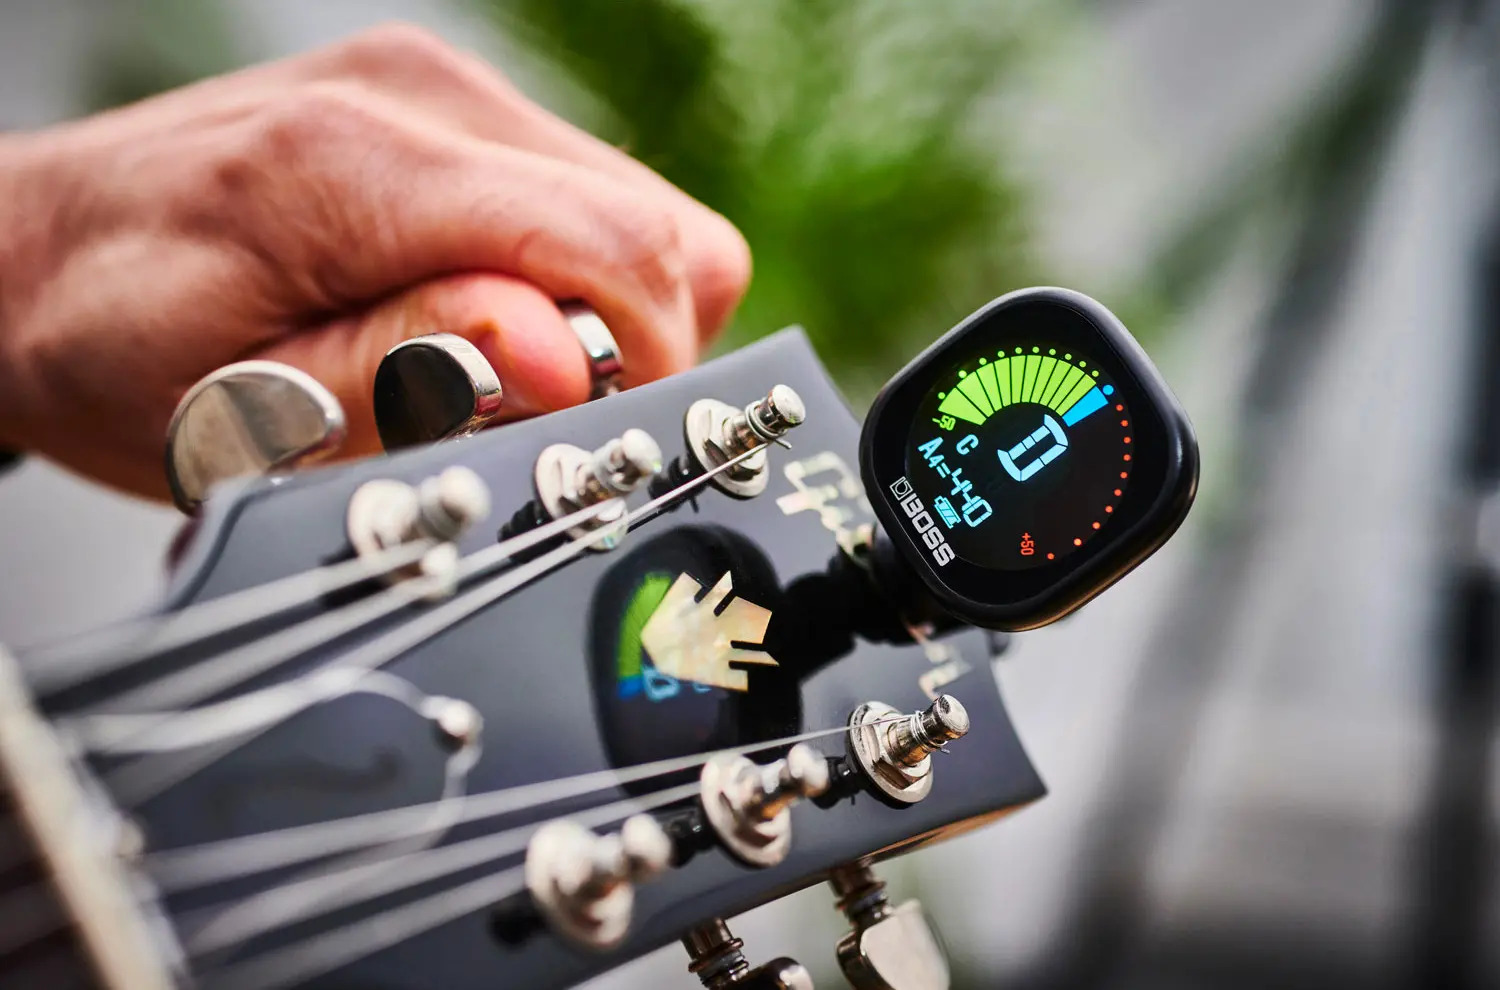
\includegraphics[width=\textwidth]{../Images/guitar-tuning.jpg}
    \captionof{figure}{Tuning a guitar \cite{Tuning}}
    \label{fig:tuning}
\end{minipage}

Another tuning options relies on the previously mentioned difference in pitch between the string. In \ref{fig:guitar_relative_tuning} you see which positions on the neck have the same pitch as the thinner string next to it.

\begin{figure}[h]
    \centering
    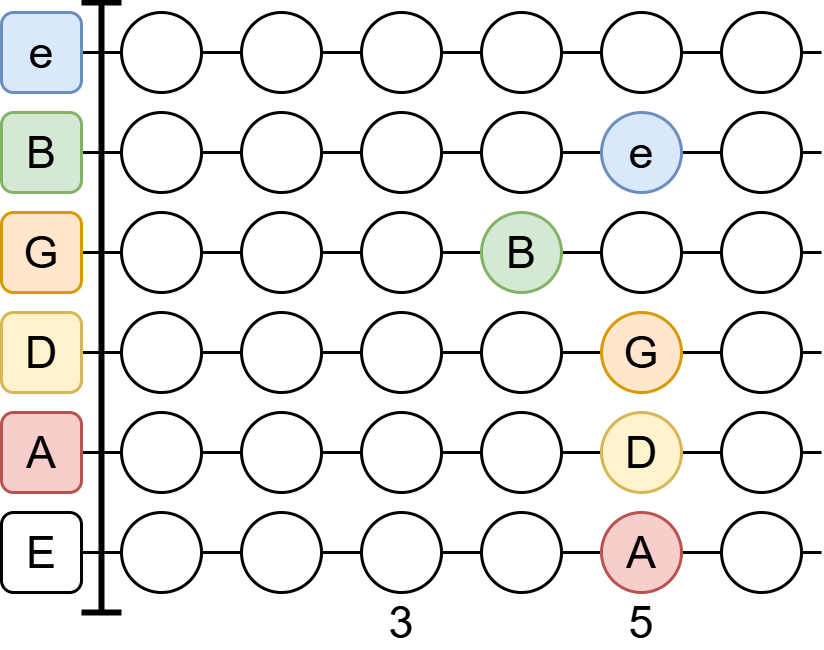
\includegraphics[width=0.5\textwidth]{../Images/GuitarRelativeTuning.png}
    \caption{Relative tuning}
    \label{fig:guitar_relative_tuning}
\end{figure}
